\setlength{\footskip}{8mm}
\addcontentsline{toc}{chapter}{Appendix C: Additional Result Images}

\begin{center}
{\large \bf Appendix C\\ \vskip 1em Additional Result Images\\ \vskip 1em}
\end{center}

This appendix provides additional qualitative material used to support the evaluation in Chapter~\ref{ch:results}. The appendix does not introduce new claims; it documents the visual evidence available in the thesis folder and clarifies the status of examples whose complete result images are not included in the local LaTeX project.

\section*{C.1 Apple Pipeline Result}

The apple example is the clearest visual support for the proposed primitive-translation pipeline. It combines explicit displacement, hard warp initialization, background restoration, and sharp compositing.

\begin{figure}[h]
  \centering
  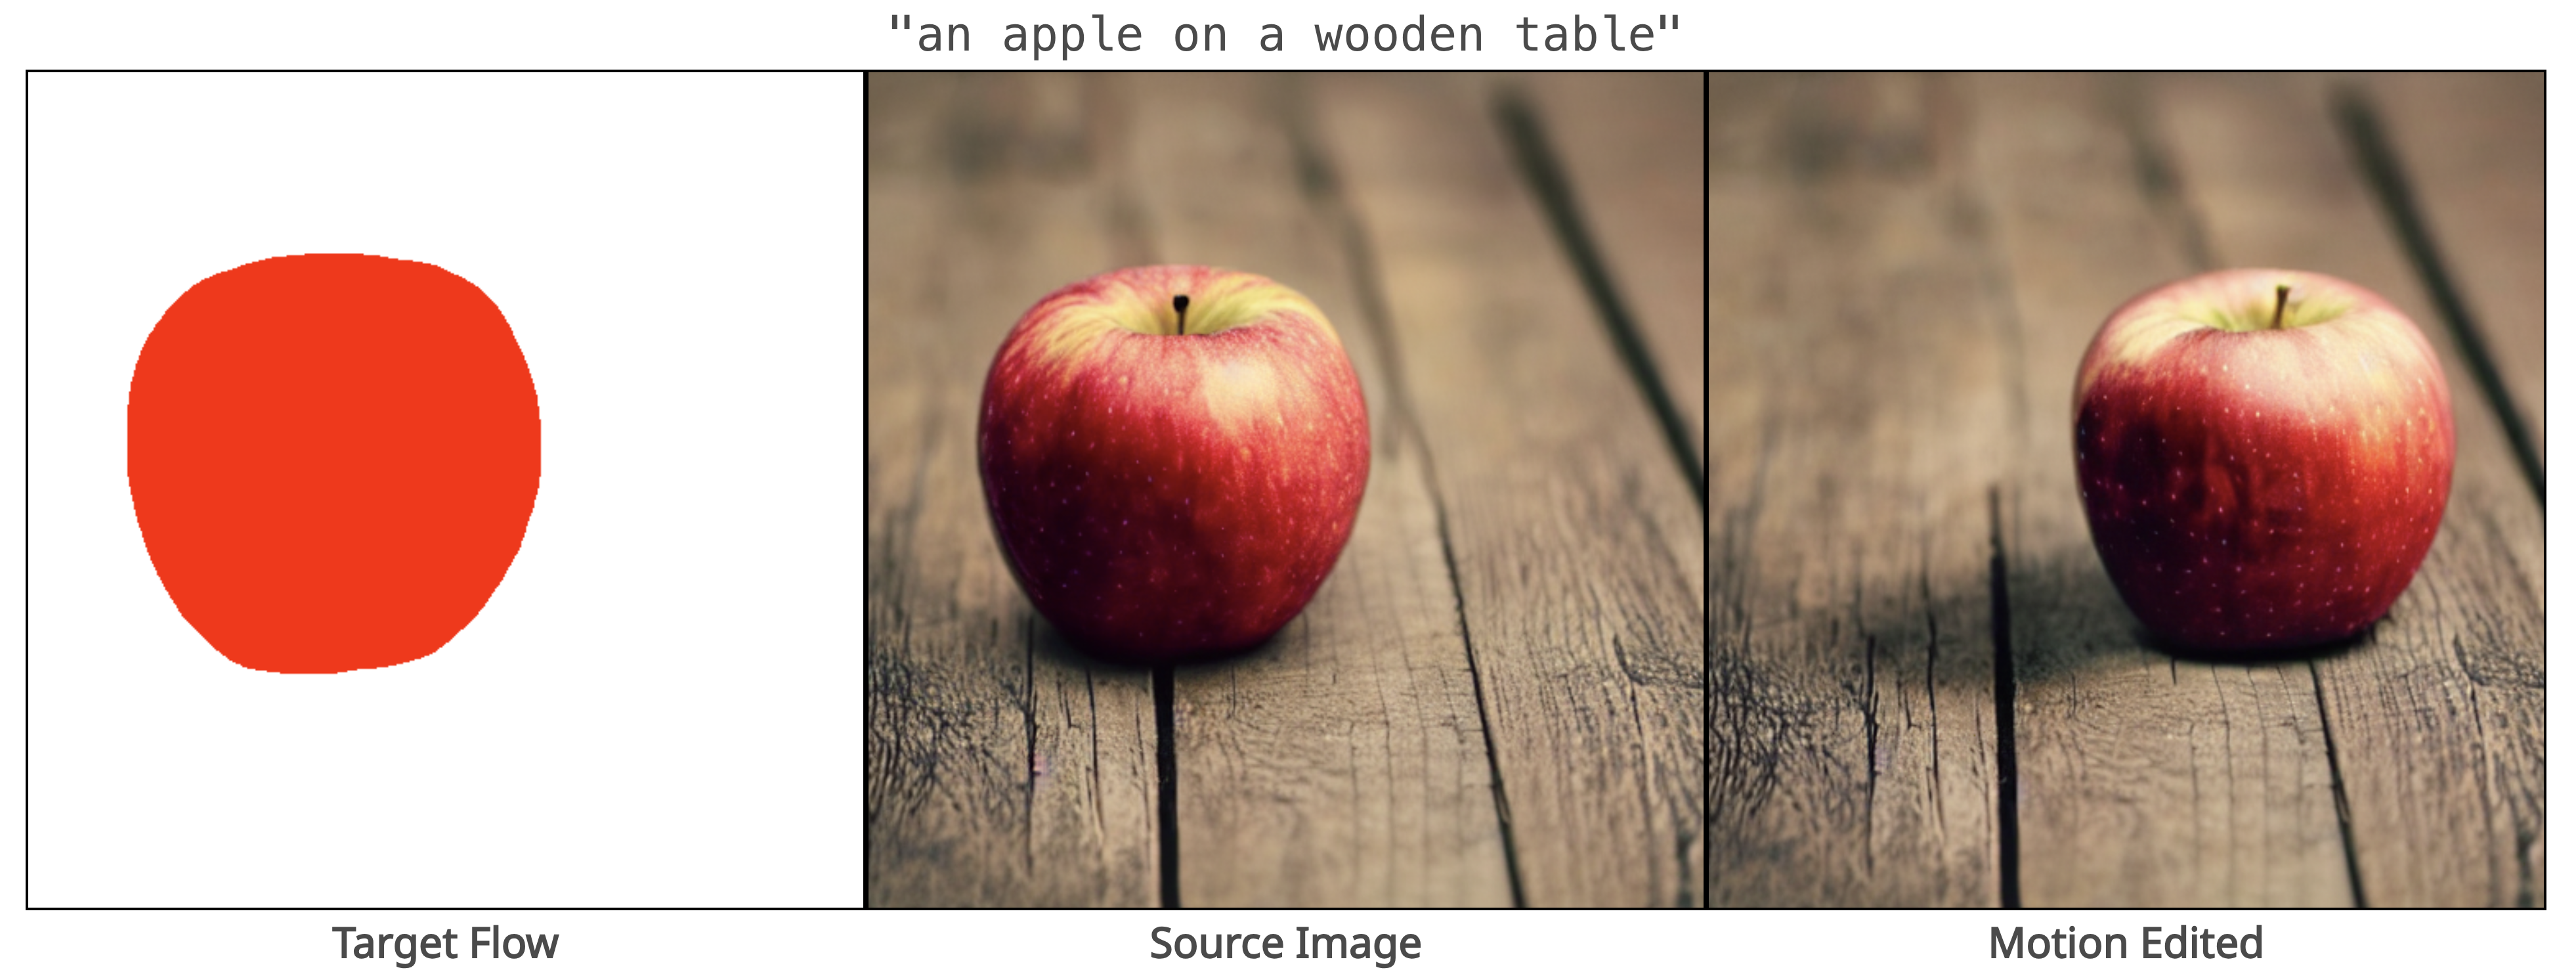
\includegraphics[width=5.6in]{figures/apple_pipeline_asset.png}
  \caption{Apple result asset used as the main qualitative evidence for controllable rigid object translation.}
  \label{fig:appendix-apple}
\end{figure}

\section*{C.2 Apple Ablation Grids}

The final apple ablation contains five variants over three seeds. Figure~\ref{fig:appendix-apple-ablation-final} shows the final saved image for each run. Rows correspond to seeds 0, 1, and 2. Columns correspond to warp-inpaint-only, original Motion Guidance, diffusion without RAFT, diffusion with RAFT, and the full pipeline.

\begin{figure}[p]
  \centering
  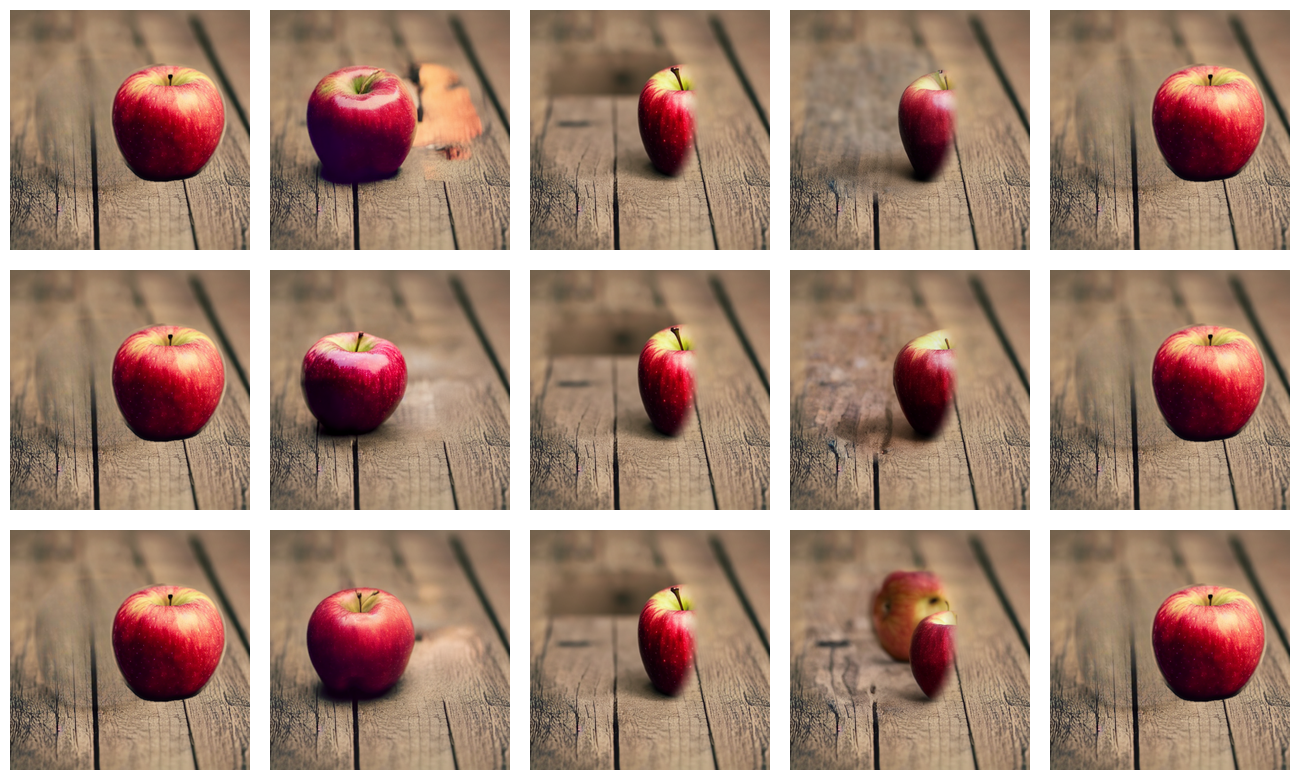
\includegraphics[width=5.9in]{figures/apple_ablation_final_grid.png}
  \caption{Final outputs from the apple ablation. This grid supports the qualitative comparison in Chapter~\ref{ch:results}.}
  \label{fig:appendix-apple-ablation-final}
\end{figure}

Figure~\ref{fig:appendix-apple-ablation-pre} shows pre-composite diffusion outputs for the primitive diffusion variants. It is included because it separates diffusion behavior from final deterministic compositing.

\begin{figure}[p]
  \centering
  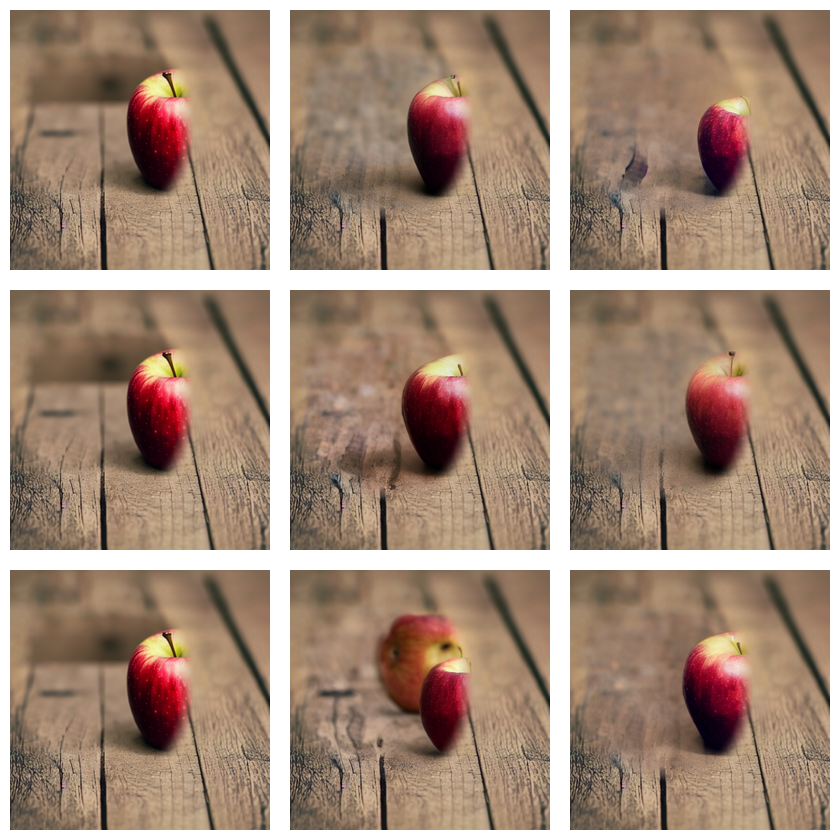
\includegraphics[width=5.7in]{figures/apple_ablation_pre_composite_grid.png}
  \caption{Pre-composite outputs for primitive diffusion variants. Rows are seeds 0--2; columns are no-RAFT diffusion, RAFT-guided diffusion, and the full-pipeline pre-composite output.}
  \label{fig:appendix-apple-ablation-pre}
\end{figure}

\section*{C.3 Additional Generated Cases}

Figure~\ref{fig:appendix-teapot-extra} shows the additional teapot translation case. This example uses the same contained-translation path as the full apple pipeline, so the final column is a hybrid output that combines diffusion-stage processing with deterministic restoration and source-object compositing.

\begin{figure}[p]
  \centering
  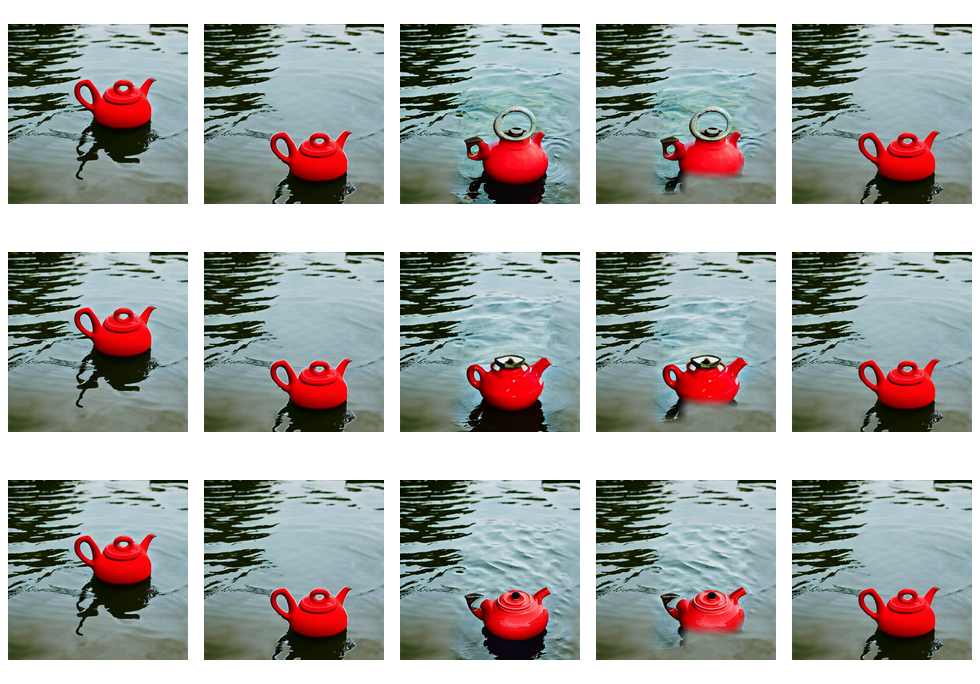
\includegraphics[width=5.9in]{figures/teapot_full_pipeline_grid.png}
  \caption{Additional teapot translation runs over seeds 0--2. Columns show source, warped initialization, decoded diffusion output, and final composited output.}
  \label{fig:appendix-teapot-extra}
\end{figure}

Figure~\ref{fig:appendix-tree-extra} shows the additional tree file-flow squeeze case. This case is included as a stress example. Seed 2 is the cleanest representative output, while seeds 0 and 1 show stronger deformation and texture variation.

\begin{figure}[p]
  \centering
  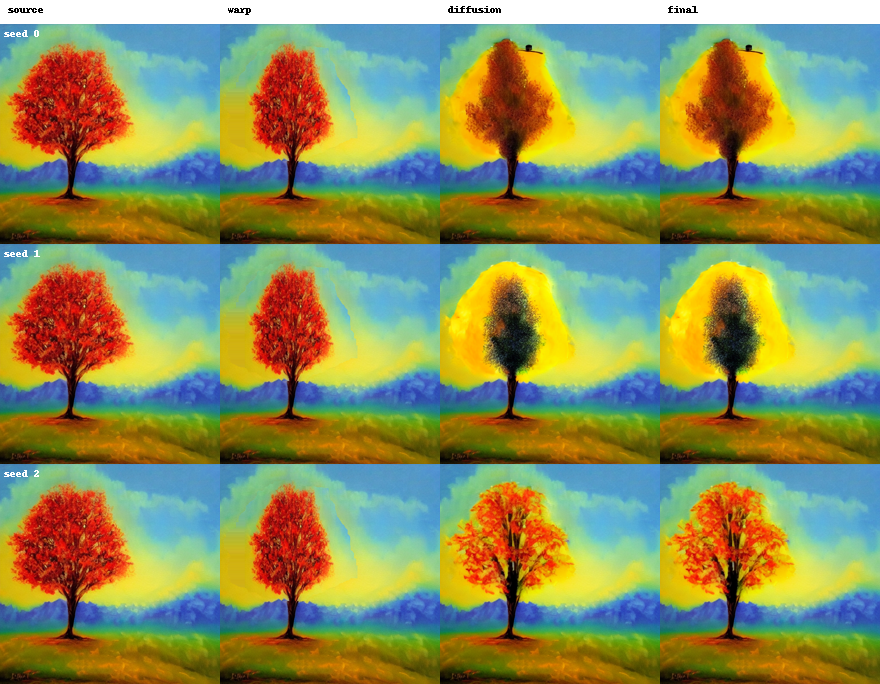
\includegraphics[width=5.9in]{figures/tree_full_pipeline_grid.png}
  \caption{Additional tree file-flow squeeze runs over seeds 0--2. The case is useful for diagnosing non-rigid/file-flow behavior, not for claiming polished non-rigid editing.}
  \label{fig:appendix-tree-extra}
\end{figure}

\section*{C.4 Excluded Presentation Assets}

The repository contains woman and topiary images used by an optional presentation mode. The application can load these assets directly after sampling, so they are deliberately omitted from this results appendix and do not support algorithmic claims.

\section*{C.5 Additional Example Status}

Table~\ref{tab:appendix-result-status} summarizes the status of the examples discussed in the thesis. It distinguishes included evidence, documented configurations, presentation assets, and unavailable examples.

\begin{table}[p]
  \centering
  \scriptsize
  \caption{Status of additional qualitative examples.}
  \label{tab:appendix-result-status}
  \renewcommand{\arraystretch}{1.15}
  \begin{tabular}{p{0.85in}|p{1.15in}|p{1.4in}|p{1.75in}}
    \hline
    \textbf{Example} & \textbf{Category} & \textbf{Image Availability} & \textbf{Use in Thesis} \\ \hline \hline
    Apple & Primitive rigid translation & 15 ablation runs included & Main quantitative and qualitative evidence \\ \hline
    Teapot & Primitive rigid translation & Three generated seeds included & Additional contained-translation evidence \\ \hline
    Tree & File-flow squeeze & Three generated seeds included & Stress case for non-rigid/file-flow behavior \\ \hline
    Lion & Primitive translation & Smoke output only & Excluded from main evidence because translation clips at the image boundary \\ \hline
    Woman & Shipped presentation asset & Omitted from results & Excluded from evaluation \\ \hline
    Topiary & Shipped presentation asset & Omitted from results & Excluded from evaluation \\ \hline
    Cat & Presentation asset only & Not a complete runnable dataset & Excluded from final evaluation \\ \hline
  \end{tabular}
\end{table}

\section*{C.6 Interpretation}

The appendix contains the directly inspectable apple ablation outputs and the additional teapot and tree generated runs. The remaining presets do not add empirical evidence in the local package. Cat is also excluded because its complete input folder, flow, mask, inversion latent, and cached latents are unavailable.
